\problemname{Grid Volleyball}
Grid Volleyball is played with two players in each team (like beach volleyball) but the players can only hit the ball when standing on a grid point.
When a player is to hit the ball, they must be ``close enough'' to where the ball is supposed to land, move there, and then hit it.
Only the player who is going to hit the ball is allowed to move.
The player decides on a grid point to which they will hit the ball, either on their own side of the net (a ``pass'') or on the opposing team's (a ``smash'').
The ball always lands on that grid point and can not be intercepted on the way.
If there is no player who can move to the grid point to where it was aimed, the team on whose side the ball lands loses.
As in beach volleyball, the ball may be hit at most three times before crossing the net (two passes and a smash) and the same person may not hit the ball twice in a row.
The first hit (the serve) must always be made from one of the corners of the field and be a smash.
It's decided that the first player ($A1$) of team $A$ serves.

Write a program that, given the size of the playing field and the four players' properties, computes which team wins if playing optimally.
If no team can force a win, the ball will be live forever which we consider a tie.

The net is transparent, so the players know where the opponents are before hitting (but remember a player may not move unless it's to hit the ball).
The game starts in the following way.
First team $A$ assumes their positions: $A1$ in a corner and $A2$ on an arbitrary position.
Afterwards, $B1$ and $B2$ assumes arbitrary positions, while $A$ may not move.
Finally, $A$ serves and the game is afoot.
The players move independently of each other, and may be on the same grid point.
However, they may not step outside of the field or into the opponent's half of the field.

\begin{figure}[h]
    \centering
    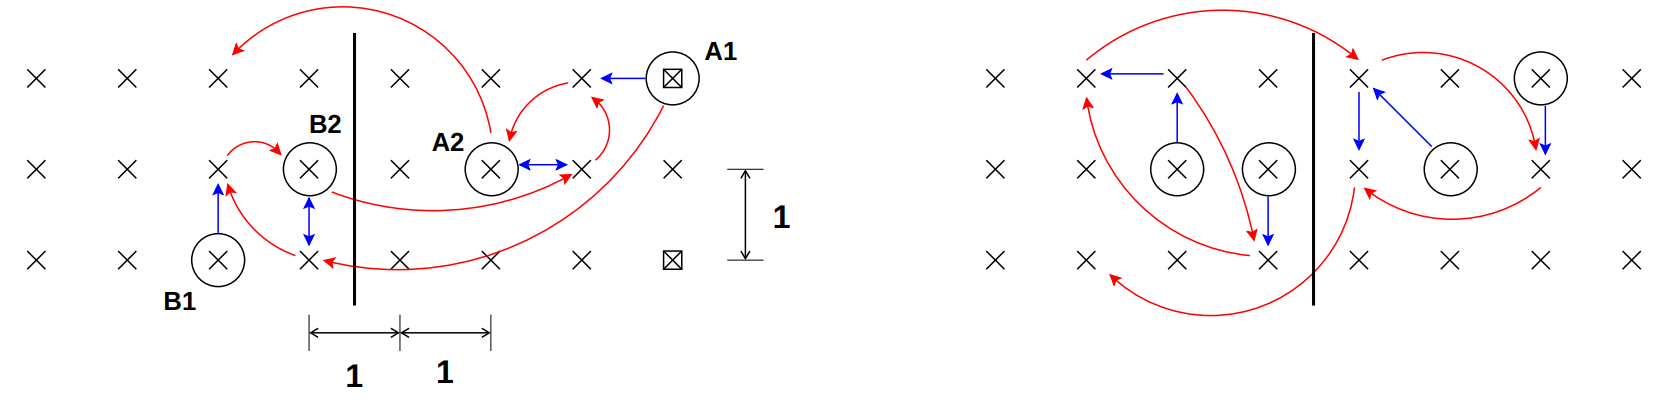
\includegraphics[width=1.0\textwidth]{grid}
    \caption{
        A possible game sequence of example $4$, with optimal play from both teams, i.e. team $A$ plays in such a way that they have a forced win with at most $5$ smashes in total while team $B$ players in such a way that team $A$ can't win after less than $5$ smashes.
        There are several other optimal ways to play.
        To the left the field is shown with the grid points marked by crosses and the two possible serve points with squares around the crosses.
        Also, an optimal starting position is displayed for the teams.
        Furthermore the path of the ball is showed with red arrows, while the players' movements are showed with blue arrows.
        For clarity, the play has been split into two pictures so that the left one shows the play up to and including the third smash, while the right figure shows the remainder of the game, including $A$ hitting the final smash that no player of team $B$ can catch.
    }
\end{figure}

\section*{Input}
The first line contains the integers $x$ ($2 \le X \le 4$) and $y$ ($2 \le Y \le 3$), the number of grid points on the $x$- and $y$-axis on each half of the field (see the figure).

Then four lines follow describing the players in the order $A1$, $A2$, $B1$ and $B2$.
Each line consists of two integers $F$ ($0 \le F \le 25$) and $S$ ($0 \le S \le 5$), where $\sqrt{F}$ is the greatest distance a player can hit the ball and $\sqrt{S}$ is the maximum distance the player can run to make a hit, i.e. the maximum distance the player can be from where the ball will land to reach it on time.

\section*{Output}
First output the result for team $A$: \texttt{win}, \texttt{loss} or \texttt{tie}.
If team $A$ wins, output the minimum number of smashes (for both teams) that team $A$ needs before it can win (this will be odd).
If team $A$ loses, instead output the minimum number of smashes (for both teams) that team $B$ needs before it can win (this will be even).
For a tie, no number should be output.

\section*{Scoring}
Your solution will be tested on a set of test case groups.
To get the points for a group, you need to pass all the test cases in the group.

\textbf{Note:} if your program only computes the result correctly but outputs an incorrect number of smashes you will receive $30$ points for a group.

\noindent
\begin{tabular}{| l | l | p{12cm} |}
  \hline
  \textbf{Group} & \textbf{Point value} & \textbf{Constraints} \\ \hline
  $1$    & $50$        & One of the teams has a forced win.\\ \hline 
  $2$    & $50$        & No additional constraints. \\ \hline 
\end{tabular}
